\section{Conception Matérielle}
Pour mettre en oeuvre les différentes parties du projet combinatoires et séquentielles, nous avons du passer par des étapes d'analyses comportementales de chaque blocs à réaliser pour ainsi créer des composants simples pouvant être utiliser à la composition de fonctions plus complexes plus tard. L'implémentation de chaque composants a été réalisée grâce au langage VHDL sur le logiciel de développement Quartus.

Ainsi nous avons réalisé différentes "boîtes" de composants simples pour réaliser des fonctions entières, et plus complexes, contenant les blocs simples.

\subsection{Réalisation fonction simple - Gestion anémomètre}
La fonction réalisant l'acquisition de la vitesse du vent (0 à 250 Km/h) se fait à l'aide d'un anémomètre qui sert de transducteur convertissant la vitesse du vent en fréquence variable (0 à 250 Hz). 
\vspace{0.5cm}\\
Le composant doit fonctionner en deux modes :
\begin{enumerate}
    \item Mode continu, dans ce mode le système actualise l'acquisition toutes les secondes de la vitesse du vent. Pour cela l'entrée "Continu" doit être à 1. 
    \item Mode mono-coup, dans ce mode le système effectue qu'une seule acquisition lorsque "Start/Stop" est activé. Une fois "data\_valide" envoyé le système remet les entrées "Start/Stop" et "data\_valide" à zéro après une acquisition et attend la prochaine entrée "Start/Stop".
\end{enumerate}
\vspace{0.5cm}
La figure 3 représente la décomposition des composants utilisés pour la réalisation du bloc "Captage direction vent". 

\begin{figure}[h]
    \begin{center}
      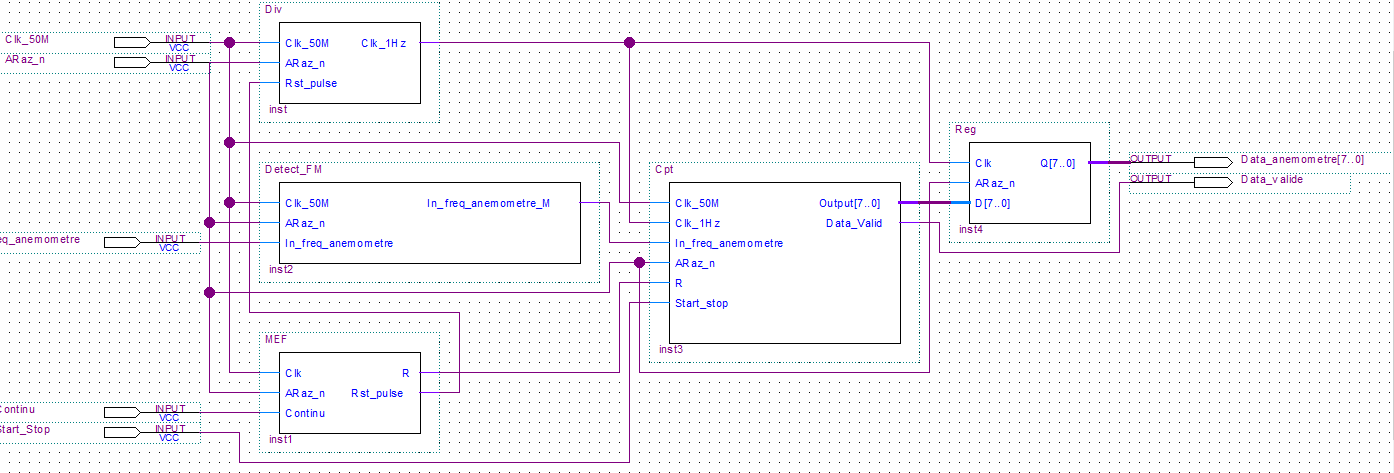
\includegraphics[width=\textwidth]{images/captation.png}
      \caption{Diagramme fonctionnel du circuit "Captation vitesse vent"}
    \end{center}
  \end{figure}

  Le composant "Div" fournit une horloge de 1 Hz à partir de l'horloge 50 MHz donnée par la clock du FPGA. L'horloge de 1 Hz sera utilisée pour l'acquisition de la fréquence de l'anémomètre toutes les secondes.

\newpage

  Le deuxième composant "Detect\_FM" est en charge de détecter les fronts montants sortant de l'anémomètre pour transformer la fréquence générée en Hertz en une donnée interprétable par le composant "Cpt".\\\newline
  Le composant "Cpt" va permettre de récupérer la quantité de fronts montants comptés par le composant "Detect\_FM", toutes les secondes quand le composant sera en mode continue et une seule fois lors du mode mono-coup.\\\newline
  Le composant "Reg" permettant de stocker la valeur de la fréquence convertie dans un registre ce qui va permettre de venir traiter ou effectuer des calculs une fois celle-ci acquise (ici dans le MCU qui sera réalisé prochainement).\\\newline
  Le composant "MEF" est chargé de gérer le mode de fonctionnement du circuit (METTRE MEF)


  \newpage

  \subsection{Réalisation fonction complexe - Gestion vérin}

  Cette circuit est composé de 3 fonctions principales qui vont permettre le pilotage du vérin qui contrôle la barre franche du voilier :
\begin{enumerate}
    \item Une gestion d'un signal PWM effectué par le process "PWM". 
    \item Un contrôle des butées réalisé par le process "Gestion\_Butée".
    \item Une machine à états pour la gestion du convertisseur MCP3201.
\end{enumerate} 

  \begin{figure}[h]
    \begin{center}
      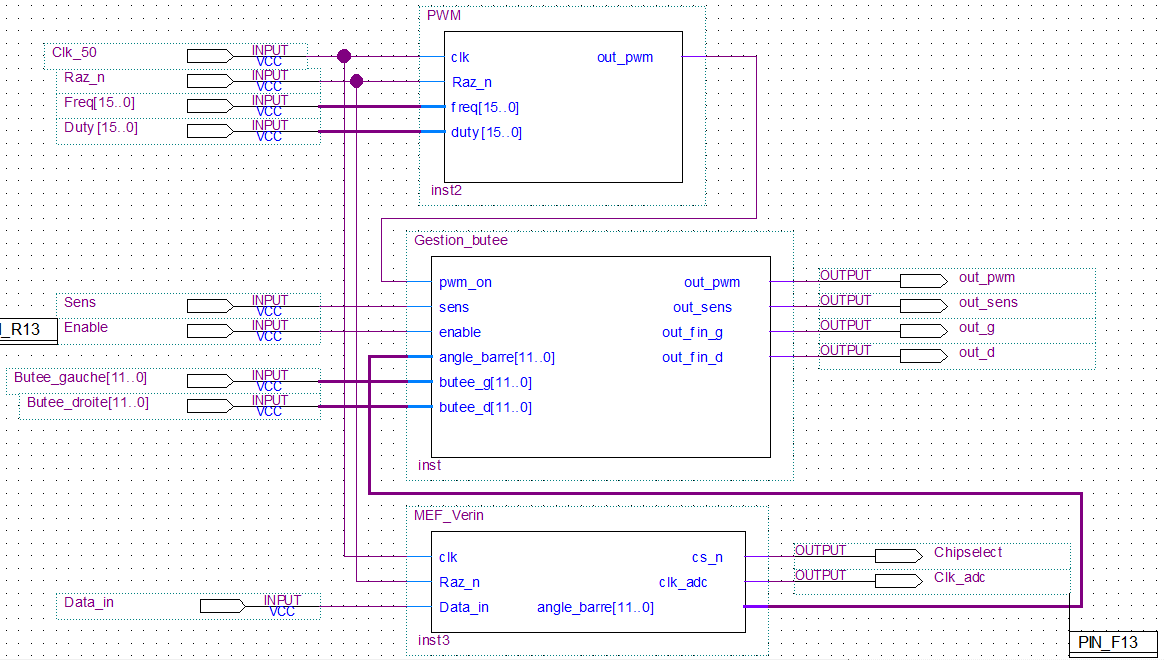
\includegraphics[width=\textwidth]{images/verin.png}
      \caption{Diagramme fonctionnel du circuit "Actionnement Barre"}
    \end{center}
  \end{figure}

  Le premier composant "PWM".\\\newline
  Le composant "Gestion\_Butée".\\\newline
  Le composant "MEF" est chargé de gérer le mode de fonctionnement du circuit (METTRE MEF)